\documentclass[tikz]{standalone}
\usetikzlibrary{arrows,backgrounds}
\tikzstyle{background grid}=[draw, step=0.2cm, gray, very thin]

% Colors
\colorlet{veccol}{black!30}
% Reference frame axis styles
\tikzstyle{vec}=[-stealth,thick,line cap=round,scale=2]

\begin{document}

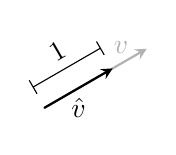
\begin{tikzpicture}
  % [show background grid]
  \coordinate (O) at (0,0);
  \coordinate (A) at (30:1.5);
  \coordinate (B) at (30:1);
  % Vectors
  % \path (A) -- (O) -- (B)
  % pic ["\(\alpha\)",draw,angle radius=10mm] {angle=A--O--B};
  \draw[vec,veccol] (O) -- node [above,near end] {\(v\)} (A);
  \draw[vec] (O) -- node [below] {\(\hat{v}\)} (B);
  % Set first coordinate at 2 mm away 120 deg from "O" and second at 1 unit
  % and 30 deg from the first, hence matching vector
  \draw[Bar-Bar] (O) ++(120:3mm) -- node [above,sloped] {1} +(30:1);
  \useasboundingbox ([shift={(-4\pgflinewidth,0)}]
  current bounding box.south west) -- (current bounding box.north east);
\end{tikzpicture}

\end{document}


%%% Local Variables:
%%% mode: latex
%%% TeX-master: t
%%% End:
